% Options for packages loaded elsewhere
\PassOptionsToPackage{unicode}{hyperref}
\PassOptionsToPackage{hyphens}{url}
%
\documentclass[
]{article}
\usepackage{amsmath,amssymb}
\usepackage{lmodern}
\usepackage{iftex}
\ifPDFTeX
  \usepackage[T1]{fontenc}
  \usepackage[utf8]{inputenc}
  \usepackage{textcomp} % provide euro and other symbols
\else % if luatex or xetex
  \usepackage{unicode-math}
  \defaultfontfeatures{Scale=MatchLowercase}
  \defaultfontfeatures[\rmfamily]{Ligatures=TeX,Scale=1}
\fi
% Use upquote if available, for straight quotes in verbatim environments
\IfFileExists{upquote.sty}{\usepackage{upquote}}{}
\IfFileExists{microtype.sty}{% use microtype if available
  \usepackage[]{microtype}
  \UseMicrotypeSet[protrusion]{basicmath} % disable protrusion for tt fonts
}{}
\makeatletter
\@ifundefined{KOMAClassName}{% if non-KOMA class
  \IfFileExists{parskip.sty}{%
    \usepackage{parskip}
  }{% else
    \setlength{\parindent}{0pt}
    \setlength{\parskip}{6pt plus 2pt minus 1pt}}
}{% if KOMA class
  \KOMAoptions{parskip=half}}
\makeatother
\usepackage{xcolor}
\usepackage[margin=1in]{geometry}
\usepackage{longtable,booktabs,array}
\usepackage{calc} % for calculating minipage widths
% Correct order of tables after \paragraph or \subparagraph
\usepackage{etoolbox}
\makeatletter
\patchcmd\longtable{\par}{\if@noskipsec\mbox{}\fi\par}{}{}
\makeatother
% Allow footnotes in longtable head/foot
\IfFileExists{footnotehyper.sty}{\usepackage{footnotehyper}}{\usepackage{footnote}}
\makesavenoteenv{longtable}
\usepackage{graphicx}
\makeatletter
\def\maxwidth{\ifdim\Gin@nat@width>\linewidth\linewidth\else\Gin@nat@width\fi}
\def\maxheight{\ifdim\Gin@nat@height>\textheight\textheight\else\Gin@nat@height\fi}
\makeatother
% Scale images if necessary, so that they will not overflow the page
% margins by default, and it is still possible to overwrite the defaults
% using explicit options in \includegraphics[width, height, ...]{}
\setkeys{Gin}{width=\maxwidth,height=\maxheight,keepaspectratio}
% Set default figure placement to htbp
\makeatletter
\def\fps@figure{htbp}
\makeatother
\setlength{\emergencystretch}{3em} % prevent overfull lines
\providecommand{\tightlist}{%
  \setlength{\itemsep}{0pt}\setlength{\parskip}{0pt}}
\setcounter{secnumdepth}{-\maxdimen} % remove section numbering
\ifLuaTeX
  \usepackage{selnolig}  % disable illegal ligatures
\fi
\IfFileExists{bookmark.sty}{\usepackage{bookmark}}{\usepackage{hyperref}}
\IfFileExists{xurl.sty}{\usepackage{xurl}}{} % add URL line breaks if available
\urlstyle{same} % disable monospaced font for URLs
\hypersetup{
  hidelinks,
  pdfcreator={LaTeX via pandoc}}

\author{}
\date{\vspace{-2.5em}}

\begin{document}

\hypertarget{analisis-exploratorio-y-estadistico}{%
\section{Analisis Exploratorio y
Estadistico}\label{analisis-exploratorio-y-estadistico}}

La preparacion del dataset se puede encontrar en GitHub,
\textbf{\texttt{pre\_step\_data\_einstein.R}}:

\begin{itemize}
\item
  Las variables se han estandardizados y centrado previamente, por al
  razon que algunos algortimos funcionan mejor con los datos escalados.
\item
  Se han removido errores, o caracteres especiales, simbolos etc.
\item
  Se han convertido columnas de \textbf{character} a \textbf{factor,
  logical} a \textbf{factor,} o algunas variables a numerical.
\item
  Se ha creado el \textbf{output}, la variable dependiente
  \textbf{care.}
\end{itemize}

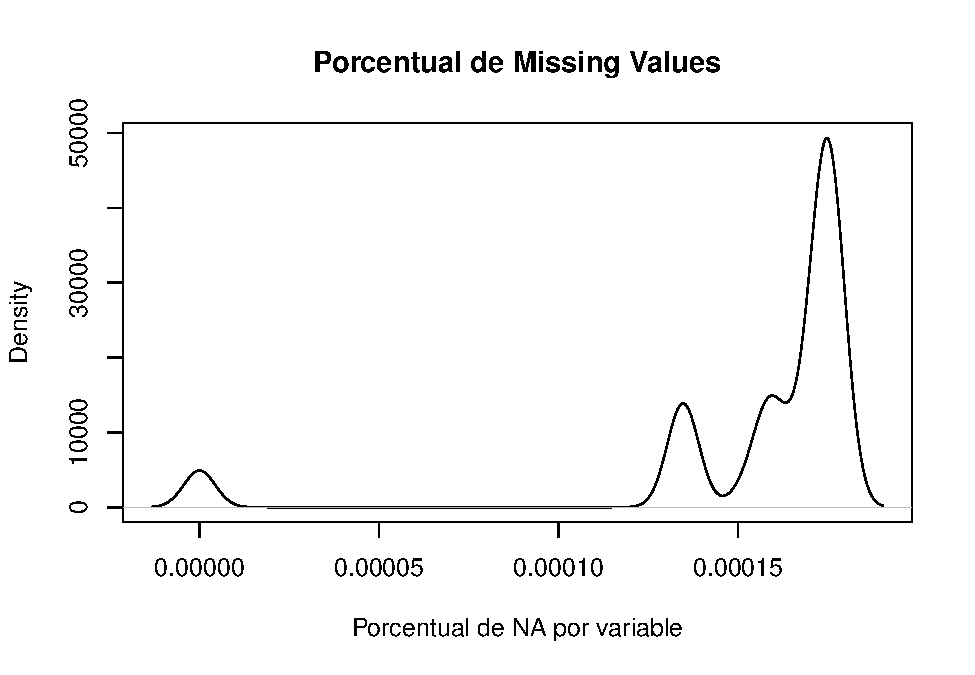
\includegraphics{04_Stat_An_files/figure-latex/unnamed-chunk-2-1.pdf}

El dataset original, tiene un alto numero de observaciones y variables
con \textbf{missing values}. Desde el dataset original se han filtrado
los datos faltantes en dos maneras.

\begin{itemize}
\item
  En el primer caso se han eliminado pacientes las vcariables que tiene
  una porcentual de 95\% de datos faltantes. Se eliminas tambien las
  observaciones que tienen por lo menos diez variables con datos.
\item
  En el otro caso se han filtrado las variables con pocos valores, y se
  han quitado las observaciones que continuaban en tener datos
  faltantes, de esta forma el dataset se ha notablemente reducido por
  numero de observaciones y variables. Pero en esto caso no hay datos
  faltantes.
\end{itemize}

Como se puede notar en la tabla aqui abajo, todavia hay datos faltantes.

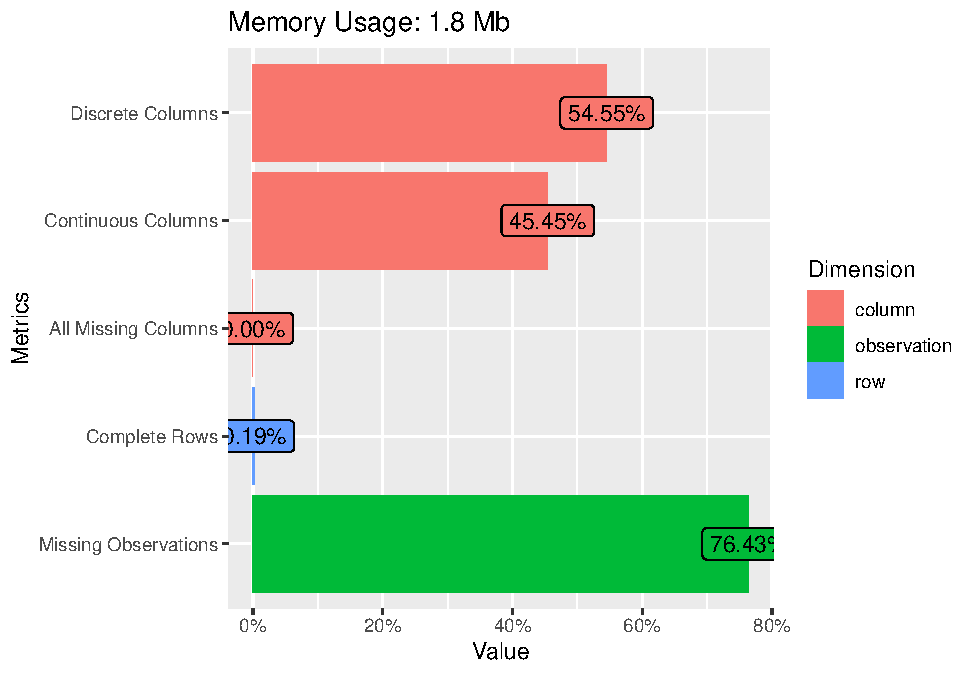
\includegraphics{04_Stat_An_files/figure-latex/unnamed-chunk-3-1.pdf}

Como se puede ver la segunda opcion es no tener datos faltantes, opcion
que se podria tener en cuenta si el numero de observacione fuese
suficientemente grande, y sin perder demasiado variables.

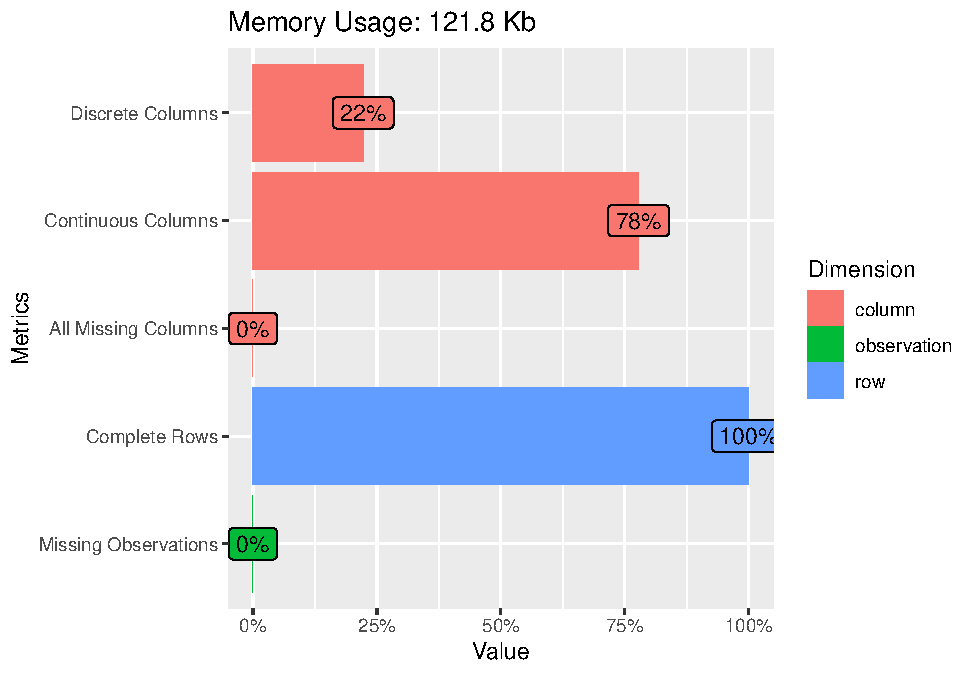
\includegraphics{04_Stat_An_files/figure-latex/unnamed-chunk-4-1.pdf}

Las variables del dataset original estan en el \textbf{Anexo -
Variables}. Las variables que quedan en los dos dataset, estan resumida
en las dos tablas estadisticas en \textbf{Anexo 2 - Tablas Estadisticas
1} para el primer caso, y \textbf{Anexo 3 - Tablas Estadisticas 2} para
el segundo caso.

\hypertarget{primer-caso}{%
\subsection{Primer caso}\label{primer-caso}}

En las dos tablas se pueden ver los casos positivos y negativos se
parado por quantiles de edad. Como Se puede notar el dataset original se
ha utilizado la poblacion y dividida por 20 grupos de tamaño igual.

En esta tabla se puede notar los casos de positividad estan repartidos
por cuantiles de edad.

\begin{longtable}[]{@{}llll@{}}
\toprule()
& negative (N=5086) & positive (N=558) & Total (N=5644) \\
\midrule()
\endhead
age\_quantile & & & \\
- 0 & 302 (5.9\%) & 1 (0.2\%) & 303 (5.4\%) \\
- 1 & 228 (4.5\%) & 1 (0.2\%) & 229 (4.1\%) \\
- 2 & 310 (6.1\%) & 5 (0.9\%) & 315 (5.6\%) \\
- 3 & 235 (4.6\%) & 17 (3.0\%) & 252 (4.5\%) \\
- 4 & 319 (6.3\%) & 47 (8.4\%) & 366 (6.5\%) \\
- 5 & 252 (5.0\%) & 44 (7.9\%) & 296 (5.2\%) \\
- 6 & 251 (4.9\%) & 33 (5.9\%) & 284 (5.0\%) \\
- 7 & 290 (5.7\%) & 30 (5.4\%) & 320 (5.7\%) \\
- 8 & 142 (2.8\%) & 27 (4.8\%) & 169 (3.0\%) \\
- 9 & 317 (6.2\%) & 44 (7.9\%) & 361 (6.4\%) \\
- 10 & 164 (3.2\%) & 27 (4.8\%) & 191 (3.4\%) \\
- 11 & 342 (6.7\%) & 40 (7.2\%) & 382 (6.8\%) \\
- 12 & 175 (3.4\%) & 27 (4.8\%) & 202 (3.6\%) \\
- 13 & 285 (5.6\%) & 30 (5.4\%) & 315 (5.6\%) \\
- 14 & 264 (5.2\%) & 39 (7.0\%) & 303 (5.4\%) \\
- 15 & 239 (4.7\%) & 35 (6.3\%) & 274 (4.9\%) \\
- 16 & 254 (5.0\%) & 29 (5.2\%) & 283 (5.0\%) \\
- 17 & 246 (4.8\%) & 19 (3.4\%) & 265 (4.7\%) \\
- 18 & 233 (4.6\%) & 26 (4.7\%) & 259 (4.6\%) \\
- 19 & 238 (4.7\%) & 37 (6.6\%) & 275 (4.9\%) \\
\bottomrule()
\end{longtable}

En esta tablas relaciona la severidad covid con los cuantiles de edad,

\begin{longtable}[]{@{}
  >{\raggedright\arraybackslash}p{(\columnwidth - 10\tabcolsep) * \real{0.1111}}
  >{\raggedright\arraybackslash}p{(\columnwidth - 10\tabcolsep) * \real{0.1709}}
  >{\raggedright\arraybackslash}p{(\columnwidth - 10\tabcolsep) * \real{0.1709}}
  >{\raggedright\arraybackslash}p{(\columnwidth - 10\tabcolsep) * \real{0.1880}}
  >{\raggedright\arraybackslash}p{(\columnwidth - 10\tabcolsep) * \real{0.2308}}
  >{\raggedright\arraybackslash}p{(\columnwidth - 10\tabcolsep) * \real{0.1282}}@{}}
\toprule()
\begin{minipage}[b]{\linewidth}\raggedright
\end{minipage} & \begin{minipage}[b]{\linewidth}\raggedright
discharged (N=5474)
\end{minipage} & \begin{minipage}[b]{\linewidth}\raggedright
regular\_ward (N=79)
\end{minipage} & \begin{minipage}[b]{\linewidth}\raggedright
semi\_intensive (N=50)
\end{minipage} & \begin{minipage}[b]{\linewidth}\raggedright
intensive\_care\_unit (N=41)
\end{minipage} & \begin{minipage}[b]{\linewidth}\raggedright
Total (N=5644)
\end{minipage} \\
\midrule()
\endhead
age\_quantile & & & & & \\
- 0 & 292 (5.3\%) & 4 (5.1\%) & 3 (6.0\%) & 4 (9.8\%) & 303 (5.4\%) \\
- 1 & 224 (4.1\%) & 1 (1.3\%) & 2 (4.0\%) & 2 (4.9\%) & 229 (4.1\%) \\
- 2 & 311 (5.7\%) & 3 (3.8\%) & 1 (2.0\%) & 0 (0.0\%) & 315 (5.6\%) \\
- 3 & 250 (4.6\%) & 1 (1.3\%) & 1 (2.0\%) & 0 (0.0\%) & 252 (4.5\%) \\
- 4 & 363 (6.6\%) & 2 (2.5\%) & 1 (2.0\%) & 0 (0.0\%) & 366 (6.5\%) \\
- 5 & 292 (5.3\%) & 2 (2.5\%) & 1 (2.0\%) & 1 (2.4\%) & 296 (5.2\%) \\
- 6 & 281 (5.1\%) & 1 (1.3\%) & 1 (2.0\%) & 1 (2.4\%) & 284 (5.0\%) \\
- 7 & 315 (5.8\%) & 3 (3.8\%) & 1 (2.0\%) & 1 (2.4\%) & 320 (5.7\%) \\
- 8 & 164 (3.0\%) & 3 (3.8\%) & 1 (2.0\%) & 1 (2.4\%) & 169 (3.0\%) \\
- 9 & 358 (6.5\%) & 1 (1.3\%) & 1 (2.0\%) & 1 (2.4\%) & 361 (6.4\%) \\
- 10 & 186 (3.4\%) & 3 (3.8\%) & 1 (2.0\%) & 1 (2.4\%) & 191 (3.4\%) \\
- 11 & 373 (6.8\%) & 4 (5.1\%) & 2 (4.0\%) & 3 (7.3\%) & 382 (6.8\%) \\
- 12 & 192 (3.5\%) & 5 (6.3\%) & 2 (4.0\%) & 3 (7.3\%) & 202 (3.6\%) \\
- 13 & 304 (5.6\%) & 6 (7.6\%) & 4 (8.0\%) & 1 (2.4\%) & 315 (5.6\%) \\
- 14 & 292 (5.3\%) & 5 (6.3\%) & 2 (4.0\%) & 4 (9.8\%) & 303 (5.4\%) \\
- 15 & 261 (4.8\%) & 6 (7.6\%) & 4 (8.0\%) & 3 (7.3\%) & 274 (4.9\%) \\
- 16 & 275 (5.0\%) & 4 (5.1\%) & 2 (4.0\%) & 2 (4.9\%) & 283 (5.0\%) \\
- 17 & 254 (4.6\%) & 8 (10.1\%) & 2 (4.0\%) & 1 (2.4\%) & 265 (4.7\%) \\
- 18 & 243 (4.4\%) & 7 (8.9\%) & 4 (8.0\%) & 5 (12.2\%) & 259 (4.6\%) \\
- 19 & 244 (4.5\%) & 10 (12.7\%) & 14 (28.0\%) & 7 (17.1\%) & 275
(4.9\%) \\
\bottomrule()
\end{longtable}

\hypertarget{segundo-caso}{%
\subsection{Segundo caso}\label{segundo-caso}}

Es mas evidente con leste dataset como los quantiles mas altos tengan
mas casos de positividad, y de necesidad de cuidado intensivo.,

\begin{longtable}[]{@{}llll@{}}
\toprule()
& negative (N=517) & positive (N=81) & Total (N=598) \\
\midrule()
\endhead
age\_quantile & & & \\
- 0 & 11 (2.1\%) & 0 (0.0\%) & 11 (1.8\%) \\
- 1 & 8 (1.5\%) & 0 (0.0\%) & 8 (1.3\%) \\
- 2 & 18 (3.5\%) & 1 (1.2\%) & 19 (3.2\%) \\
- 3 & 18 (3.5\%) & 0 (0.0\%) & 18 (3.0\%) \\
- 4 & 27 (5.2\%) & 1 (1.2\%) & 28 (4.7\%) \\
- 5 & 17 (3.3\%) & 5 (6.2\%) & 22 (3.7\%) \\
- 6 & 27 (5.2\%) & 1 (1.2\%) & 28 (4.7\%) \\
- 7 & 23 (4.4\%) & 3 (3.7\%) & 26 (4.3\%) \\
- 8 & 13 (2.5\%) & 2 (2.5\%) & 15 (2.5\%) \\
- 9 & 41 (7.9\%) & 1 (1.2\%) & 42 (7.0\%) \\
- 10 & 20 (3.9\%) & 4 (4.9\%) & 24 (4.0\%) \\
- 11 & 37 (7.2\%) & 5 (6.2\%) & 42 (7.0\%) \\
- 12 & 17 (3.3\%) & 9 (11.1\%) & 26 (4.3\%) \\
- 13 & 38 (7.4\%) & 6 (7.4\%) & 44 (7.4\%) \\
- 14 & 29 (5.6\%) & 9 (11.1\%) & 38 (6.4\%) \\
- 15 & 29 (5.6\%) & 5 (6.2\%) & 34 (5.7\%) \\
- 16 & 31 (6.0\%) & 3 (3.7\%) & 34 (5.7\%) \\
- 17 & 31 (6.0\%) & 7 (8.6\%) & 38 (6.4\%) \\
- 18 & 31 (6.0\%) & 10 (12.3\%) & 41 (6.9\%) \\
- 19 & 51 (9.9\%) & 9 (11.1\%) & 60 (10.0\%) \\
\bottomrule()
\end{longtable}

\begin{longtable}[]{@{}
  >{\raggedright\arraybackslash}p{(\columnwidth - 10\tabcolsep) * \real{0.1130}}
  >{\raggedright\arraybackslash}p{(\columnwidth - 10\tabcolsep) * \real{0.1652}}
  >{\raggedright\arraybackslash}p{(\columnwidth - 10\tabcolsep) * \real{0.1739}}
  >{\raggedright\arraybackslash}p{(\columnwidth - 10\tabcolsep) * \real{0.1913}}
  >{\raggedright\arraybackslash}p{(\columnwidth - 10\tabcolsep) * \real{0.2348}}
  >{\raggedright\arraybackslash}p{(\columnwidth - 10\tabcolsep) * \real{0.1217}}@{}}
\toprule()
\begin{minipage}[b]{\linewidth}\raggedright
\end{minipage} & \begin{minipage}[b]{\linewidth}\raggedright
discharged (N=470)
\end{minipage} & \begin{minipage}[b]{\linewidth}\raggedright
regular\_ward (N=57)
\end{minipage} & \begin{minipage}[b]{\linewidth}\raggedright
semi\_intensive (N=42)
\end{minipage} & \begin{minipage}[b]{\linewidth}\raggedright
intensive\_care\_unit (N=29)
\end{minipage} & \begin{minipage}[b]{\linewidth}\raggedright
Total (N=598)
\end{minipage} \\
\midrule()
\endhead
age\_quantile & & & & & \\
- 0 & 9 (1.9\%) & 0 (0.0\%) & 1 (2.4\%) & 1 (3.4\%) & 11 (1.8\%) \\
- 1 & 5 (1.1\%) & 0 (0.0\%) & 2 (4.8\%) & 1 (3.4\%) & 8 (1.3\%) \\
- 2 & 16 (3.4\%) & 2 (3.5\%) & 1 (2.4\%) & 0 (0.0\%) & 19 (3.2\%) \\
- 3 & 16 (3.4\%) & 1 (1.8\%) & 1 (2.4\%) & 0 (0.0\%) & 18 (3.0\%) \\
- 4 & 25 (5.3\%) & 2 (3.5\%) & 1 (2.4\%) & 0 (0.0\%) & 28 (4.7\%) \\
- 5 & 19 (4.0\%) & 1 (1.8\%) & 1 (2.4\%) & 1 (3.4\%) & 22 (3.7\%) \\
- 6 & 27 (5.7\%) & 0 (0.0\%) & 0 (0.0\%) & 1 (3.4\%) & 28 (4.7\%) \\
- 7 & 24 (5.1\%) & 1 (1.8\%) & 1 (2.4\%) & 0 (0.0\%) & 26 (4.3\%) \\
- 8 & 13 (2.8\%) & 1 (1.8\%) & 0 (0.0\%) & 1 (3.4\%) & 15 (2.5\%) \\
- 9 & 39 (8.3\%) & 1 (1.8\%) & 1 (2.4\%) & 1 (3.4\%) & 42 (7.0\%) \\
- 10 & 20 (4.3\%) & 3 (5.3\%) & 1 (2.4\%) & 0 (0.0\%) & 24 (4.0\%) \\
- 11 & 37 (7.9\%) & 2 (3.5\%) & 2 (4.8\%) & 1 (3.4\%) & 42 (7.0\%) \\
- 12 & 19 (4.0\%) & 4 (7.0\%) & 1 (2.4\%) & 2 (6.9\%) & 26 (4.3\%) \\
- 13 & 36 (7.7\%) & 5 (8.8\%) & 3 (7.1\%) & 0 (0.0\%) & 44 (7.4\%) \\
- 14 & 28 (6.0\%) & 5 (8.8\%) & 1 (2.4\%) & 4 (13.8\%) & 38 (6.4\%) \\
- 15 & 25 (5.3\%) & 4 (7.0\%) & 4 (9.5\%) & 1 (3.4\%) & 34 (5.7\%) \\
- 16 & 28 (6.0\%) & 2 (3.5\%) & 2 (4.8\%) & 2 (6.9\%) & 34 (5.7\%) \\
- 17 & 29 (6.2\%) & 7 (12.3\%) & 1 (2.4\%) & 1 (3.4\%) & 38 (6.4\%) \\
- 18 & 26 (5.5\%) & 6 (10.5\%) & 4 (9.5\%) & 5 (17.2\%) & 41 (6.9\%) \\
- 19 & 29 (6.2\%) & 10 (17.5\%) & 14 (33.3\%) & 7 (24.1\%) & 60
(10.0\%) \\
\bottomrule()
\end{longtable}

\end{document}
